%%%%%%%%%%%%%%%%%%%%%%%%%%%%%%%%%%%%%%%%%%%%%%%%%%%%
%%%%%%%%%%%%%%%%%%%%%%%%%%%%%%%%%%%%%%%%%%%%%%%%%%%%%%%%%%%%%%%%%%%%%%
% Chapitre 4
\chapter{Chapitre 4 : Conception Détaillée}

%%%%% Intro Chapitre 4
\section*{Introduction}
\phantomsection
\addcontentsline{toc}{section}{Introduction}

\paragraph{}\begin{spacing}{2}
Dans ce chapitre, nous allons entreprendre la conception des différents diagrammes et
flux qui constituent cette application, fournissant ainsi une représentation claire et détaillée
des interactions, des processus et des composants du système.
\end{spacing}
\newpage
\section{Analyse et Conception}
\subsection{Les Acteurs du Système}
\subsection*{Apprenant (Utilisateur / Étudiant)}
L’apprenant est l’acteur principal qui utilise la plateforme pour consulter, suivre et évaluer les cours.

\subsubsection*{Rôles :}
\begin{itemize}
    \item S’inscrire et créer un profil
    \item Choisir ses centres d’intérêt  
    \item Recevoir des recommandations personnalisées
\end{itemize}
\subsection*{Système de Recommandation}
Moteur intelligent qui analyse les données de l’utilisateur (centres d’intérêt, historique, niveau, etc.) pour générer des suggestions personnalisées de cours.

\section{Diagramme de Cas d’utilisation}
\paragraph{}\begin{spacing}{1}
Le diagramme de cas d’utilisation décrit le comportement du système du point de vue utilisateur sous forme d’actions et de réactions.

Il existe deux concepts fondamentaux dans la modélisation par les cas d’utilisation :
\begin{itemize}
    \item \textbf{Les acteurs} qui agissent sur le système.
    \item \textbf{Les cas d’utilisations} qui représentent les façons dont le système est manipulé par les acteurs.
\end{itemize}

Chaque cas d’utilisation indique une fonctionnalité du système déclenchée par un acteur externe au système.

Ce genre de diagramme permet de mettre en place et de comprendre les besoins des utilisateurs.
\end{spacing}
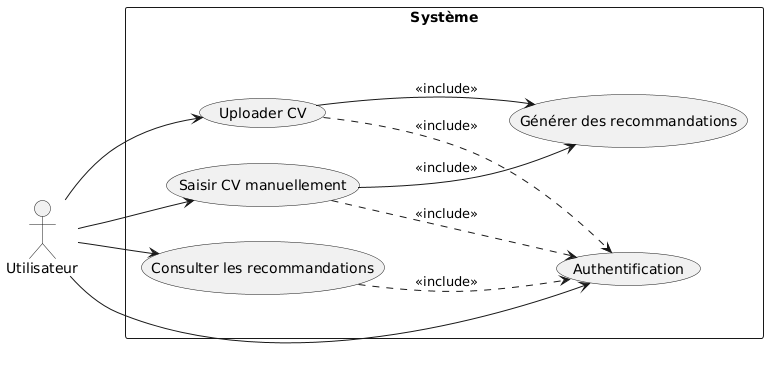
\includegraphics[width=\linewidth, height=5cm]{images/diagramme cas utilisation.png}


\section{Diagrammes de Séquence}
\paragraph{}\begin{spacing}{1}
Parmi les diagrammes intéressants d’UML, on trouve le \textbf{diagramme de séquence} qui illustre une représentation graphique des interactions entre l’acteur et le système selon un ordre chronologique dans la formulation Unified Modeling Language.

L’utilité du diagramme de séquence est de montrer les interactions d’objet dans le cadre d’un scénario de cas d’utilisation. La dimension verticale du diagramme représente le \textbf{temps}, permettant de visualiser l'enchaînement des actions dans le temps, et de spécifier la naissance et la mort d'objets.

Les périodes d'activité des objets sont symbolisées par des \textbf{rectangles}, et ces objets dialoguent à l'aide de \textbf{messages}. 

Donc, vu le service offert par les diagrammes de séquence, cette partie est consacrée à citer ceux des cas d’utilisation les plus importants dans l’application, ce qui permet de mieux voir et tracer l’enchaînement du projet.
\end{spacing}
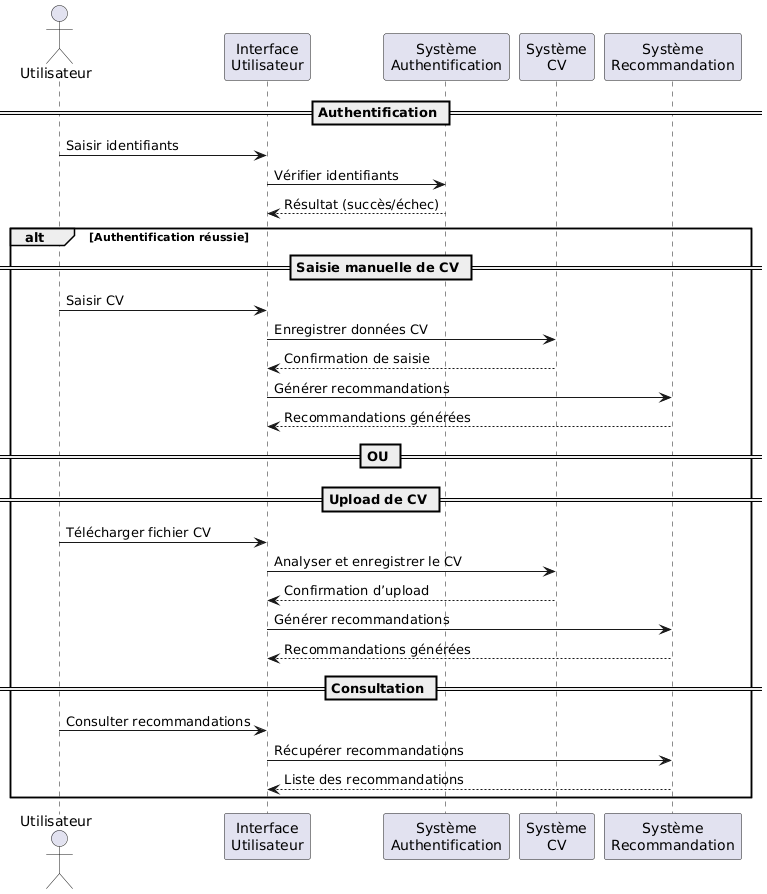
\includegraphics[width=\linewidth, height=11cm]{images/diagramme dequence.png}

\section{Diagrammes d’Activité}
\paragraph{}\begin{spacing}{1}
Le \textbf{diagramme d’activité} est l’un des diagrammes comportementaux d’UML les plus utilisés. Il permet de modéliser les différents flux de contrôle ou de données au sein d’un processus métier ou d’un scénario spécifique du système.

Il illustre la séquence des activités ou des actions réalisées par les acteurs ou les composants du système. Chaque activité représente une étape ou une opération, et les flèches indiquent la transition d’une activité à une autre.

Ce diagramme met en évidence les \textbf{conditions}, les \textbf{boucles}, les \textbf{décisions}, et permet aussi de représenter des traitements parallèles. Il est particulièrement utile pour analyser les processus métiers, décrire les algorithmes et documenter les comportements dynamiques d’un système.

Ainsi, dans cette partie, nous allons présenter les diagrammes d’activité associés aux cas d’utilisation les plus significatifs de l’application, afin de mieux visualiser les enchaînements logiques et opérationnels des différentes fonctionnalités du système.
\end{spacing}
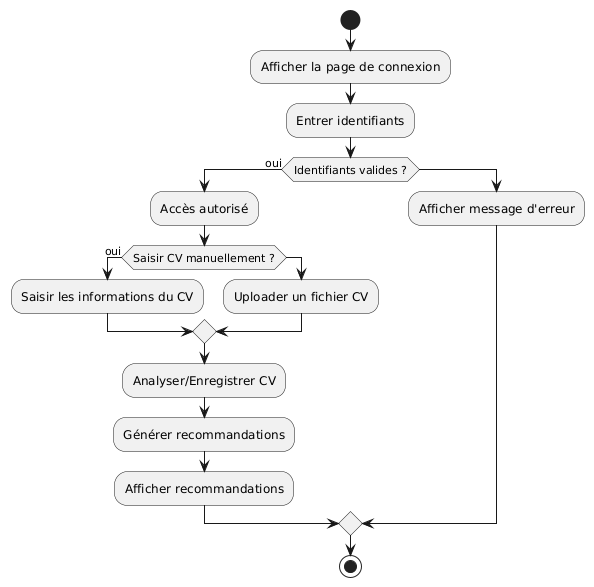
\includegraphics[width=\linewidth, height=8cm]{images/diagramme activite.png}

